\documentclass[conference]{IEEEtran}
\RequirePackage{cite}
\RequirePackage{amsmath,amssymb,amsfonts}
\RequirePackage{algorithmic}
\RequirePackage{graphicx}
\RequirePackage{textcomp}
\RequirePackage{xcolor}
\RequirePackage{hyperref}
\RequirePackage{csquotes}
\RequirePackage{listings}
\def\BibTeX{{\rm B\kern-.05em{\sc i\kern-.025em b}\kern-.08em
    T\kern-.1667em\lower.7ex\hbox{E}\kern-.125emX}}
\begin{document}

\title{Literature Review}
\author{Andrew~Fearing, Neelay~Junnarkar,  Hamza~Kamran~Khawaja}
\maketitle

\begin{abstract}
This document is for writing about the papers we find. Currently the plan is to do control of boats.
\end{abstract}

\section{Questions}
We want lane-keeping for boats. Are we doing sailboats or motorboats? It looks like motorboats are already kind of understood. I'm not exactly sure where we can contribute. Sailboats seem a lot more recent.

We need to figure out when a sailboat is controllable
\section{Search terms}
\begin{itemize}
    \item USV
    \item underactuated
    \item sailboat
    \item robotic sailboat
\end{itemize}
\section{Glossary}
\begin{itemize}
    \item USV (unmanned surface vehicles)
    \item COLREGS are rules for avoiding collisions with boats
    \item underactuated vs. fully-actuated. I believe this refers to if we can go in an arbitrary direction  \href{https://ocw.mit.edu/courses/electrical-engineering-and-computer-science/6-832-underactuated-robotics-spring-2009/readings/MIT6_832s09_read_ch01.pdf}{source}
    \item SNAME = Society of Naval Architects and Marine Engineers
\end{itemize}

\section{Control/Path Planning}
\cite{Nan2020} Data-driven robust PID control of unknown USVs*. Uses robust PID control of unknown USVs. So robust control with uncertainties.

\cite{Tan2010} Criteria and rule based obstacle avoidance for USVs explains some path-planning for boats. Splits the process into two parts: a big plan and then a local plan. It explicitly mentions lane keeping.

\cite{Yu2010} Robust path following control of an unmanned boat. They do an experiment to verify that their mixed \(\mathrm{H}_\infty / \mathrm{H}_2\) based control works. IDK what that is. Maybe look for a follow up because the conclusion says they're going to get multi-USV control working. That was back in 2010.

\cite{Dai2017} Leader-Follower Formation Control of USVs with Prescribed Performance and Collision Avoidance. This paper deals with fully actuated boats.

\cite{Velueta2019} A Strategy of Robust Control for the Dynamics of an Unmanned Surface Vehicle under Marine Waves and Currents. Uses sliding mode control. Probably a motorboat. 

\cite{HelmiAbrougui2019} Autopilot Design for an Autonomous Sailboat Based on Sliding Mode Control. Catamaran sailboat, 4 DOF model, only wind, no water disturbances. Feedback linearization for control.

\cite{Li2016} Fractional-Order PID Controller of USV Course-Keeping Using Hybrid GA-PSO Algorithm. Defines underactuated system. \enquote{In recent years, the maneuvering of underactuated surface vessels has become the focus of scholars’ attention. The underactuated system is a system that the number of control system input less than the freedom degrees of system. That means the spatial dimension of control input is less than spatial dimension of configuration. In USV control, when needing to rely on the rudder of transshipment torque and propeller longitudinal propulsion and controlling vessels in horizontal position and heading angle three degree of freedom motion, the USV control system belongs to the underactuated system.}



\section{Navigation}
\cite{Vaneck1997} Fuzzy Guidance Controller for an Autonomous Boat. An old paper on waypoint following.

 

\section{Models}
\subsection{SAILBOT Autonomous Marine Robot of Eolic Propulsion} \cite{Alves2010}  A master's thesis on an autonomous sailboat. They start with a 6-DOF model and then simplify it down to a 3-DOF model by assuming waves negligible.
\begin{figure}
    \centering
    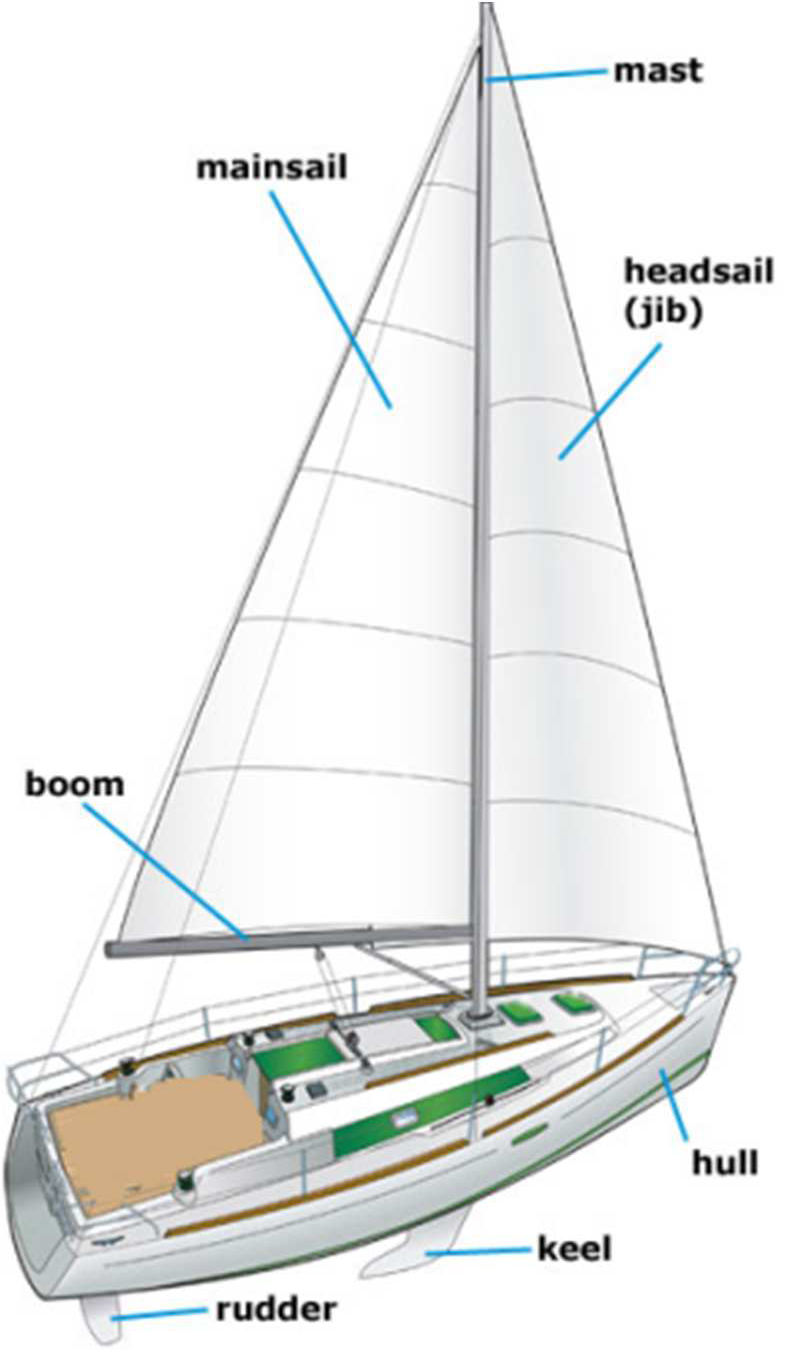
\includegraphics{documents/figures/alves_sailboat.png}
    \caption{Alves sailboat \cite{Alves2010}}
    \label{fig:alves_sailboat}
\end{figure}



\cite{Huang2017} Tries to figure out how close a boat model is from reality. Inconclusive, they only do preliminary work. Further work could be done, but it probably requires a real life boat.

\cite{Setiawan2020} Development of Dynamic Model of Autonomous Sailboat for Simulation and Control. Tries to make a dynamic model of autonomous sailboat. Might want to contrast with \cite{Buehler2018}. This is a 4-DOF model.

\cite{Buehler2018} Dynamic simulation model for an autonomous sailboat. This paper derives a dynamic model for a sailboat. There is a \href{https://github.com/simonkohaut/stda-sailboat-simulator/tree/master/src}{GitHub repo} with their Python simulation. 6-DOF model.

\cite{Paravisi2019} Unmanned Surface Vehicle Simulator with Realistic Environmental Disturbances. A paper on a ROS Kinetic simulator they made. It does currents and different boat types. There is a \href{https://github.com/disaster-robotics-proalertas/usv_sim_lsa}{GitHub repo}.

\cite{Setiawan2020} Experimental Study on the Aerodynamic Performance of Autonomous Boat with Wind Propulsion and Solar Power. From the same author who developed the dynamic model. Experimental results. Really over my head because it has to do with aerodynamics.


\cite{Sauze2006} Design and navigation of an autonomous sailboat. The authors create a sailboat model to hold a pre-determined compass course and to test the ability of the hull/sail design to cope with different points of sail.


\cite{DosSantos2020} Performance Evaluation of Propulsion Control Techniques for Autonomous Sailboat. Proposes ways to measure the performance of autonomous sailboats. Includes refs to a bunch of papers on control of sailboats.

\cite{Xiao2014} Modeling and nonlinear heading control of sailing yachts. This is pretty much what we want. Does a 4-DOF model of a sailboat. Good introduction surveys the problem.


\section{Notes}
It looks like control of sailboats is the newest thing. Robust control of fully-actuated USV's has been kind of done. So sailboats is where we can contribute without too high a bar of entry. One of the big hold ups is accurate simulation. It seems like the literature is just guessing what dynamic models fit the reality. Not even counting wind.


\section{STDA Sailboat Simulator}
This is the simulator form \cite{Buehler2018}. It prints out graphs and may be simpler to use at first. Use \lstinline{python run.py}. The package requires Python 2.7, so a conda environment YAML file is on our GitHub.


\section{Roadmap}
\begin{enumerate}
    \item Replicate 3-DOF model from \cite{Alves2010}.
    \item Use a controller to get this model through a channel.
    \item Make it more complicated with a 4- or 6-DOF model from \cite{Buehler2018} or \cite{Setiawan2020}.
    \item Add weather effects to taste. Maybe using \cite{Paravisi2019}.
\end{enumerate}

\bibliographystyle{IEEEtran}
\bibliography{refs.bib}

\end{document}
